% This is samplepaper.tex, a sample chapter demonstrating the
% LLNCS macro package for Springer Computer Science proceedings;
% Version 2.20 of 2017/10/04
%
\documentclass[runningheads]{llncs}
%
\usepackage{graphicx}
% Used for displaying a sample figure. If possible, figure files should
% be included in EPS format.
%
% If you use the hyperref package, please uncomment the following line
% to display URLs in blue roman font according to Springer's eBook style:
% \renewcommand\UrlFont{\color{blue}\rmfamily}
% For correct quotation marks (command \enquote)
\usepackage{csquotes}
\begin{document}
%
\title{Interpretable Machine Learning -- A Brief History, State-of-the-Art and Challenges\thanks{This project is funded by the Bavarian State Ministry of Science and the Arts and coordinated by the Bavarian Research Institute for Digital Transformation (bidt) and supported by the German Federal Ministry of Education and Research (BMBF) under Grant No. 01IS18036A.
The authors of this work take full responsibilities for its content.
}}
%
\titlerunning{IML - History, Methods, Challenges}
% If the paper title is too long for the running head, you can set
% an abbreviated paper title here
%
\author{Christoph Molnar\inst{1}\orcidID{0000-0003-2331-868X}}
%\and
%Second Author\inst{2,3}\orcidID{1111-2222-3333-4444} \and
%Third Author\inst{3}\orcidID{2222--3333-4444-5555}}
%
\authorrunning{Molnar}
% First names are abbreviated in the running head.
% If there are more than two authors, 'et al.' is used.
%
\institute{LMU Munich, Ludwigstr. 33, 80539 Munich, Germany
\email{christoph.molnar@gmail.com}\\
\url{https://www.slds.stat.uni-muenchen.de/people/molnar/}}
%
\maketitle              % typeset the header of the contribution
%
\begin{abstract}
  We present a brief history of interpretable machine learning (IML), give an overview of state-of-the-art interpretation methods and discuss challenges when interpreting machine learning models.
  This paper reviews IML from a methodological viewpoint, with an emphasis on what can we derive mathematically and algorithmically from an ML model.

\keywords{Interpretable Machine Learning \and Explainable Artificial Intelligence}
\end{abstract}
%
%
Interpretability is often a deciding factor when a machine learning (ML) model is used in a product, a decision process or in research.
Interpretable machine learning (IML) methods \footnote{We will be using Interpretable Machine Learning and Explainable AI exchangeably} can be used to discover knowledge, justify the model and its predictions and to control and improve the models \cite{adadi2018peeking}.
In this paper, we take a look at the historical building blocks of interpretable machine learning and give an overview of methods to interpret models.
We argue that interpretable machine learning has reached a state of usability, but some challenges remain.

\section{A Brief History of IML}
A lot of IML research happened in the last couple of years.
But learning interpretable models from data has a much longer tradition.
Linear regression models have been used back in 1800 by Gauss, Legendre and Quetelet \cite{stigler1986history,legendre1805nouvelles,gauss1809theoria,quetelet1827recherches}.
Rule-based machine learning (e.g., decision rules and trees) has been an active research area since the 1980s \cite{furnkranz2012foundations}.
A lot of machine learning research began in the second half of the 20th century with research on, for example, support vector machines in 1974 \cite{vapnik1974theory}, early important work on neural networks in the 1960s \cite{schmidhuber2015deep} and boosting in 1990 \cite{schapire1990strength}.
Interpretability has always been a companion of ML.
The random forest algorithm  \cite{breiman2001random} is an example of the early importance of interpretability and also an IML milestone.
Random forests, a black box machine learning model that often works well without tuning, came with a built-in feature importance measure, which contributed to its success.
\footnote{The random forest paper has been cited  $>60000$ times (Google Scholar; September 2020) and there are many papers improving the importance measure (\cite{strobl2008conditional,strobl2007bias,hapfelmeier2014new,ishwaran2007variable}) which are also cited frequently.}
In the 2010s came the deep learning hype, after a deep neural network won the ImageNet challenge.
A few years after that, the IML field really took off (around 2015), judging by frequency of the search terms "Interpretable Machine Learning" and "Explainable AI" on Google (Figure \ref{fig:count} right) and papers published with these terms (Figure \ref{fig:count} left).
\begin{figure}
  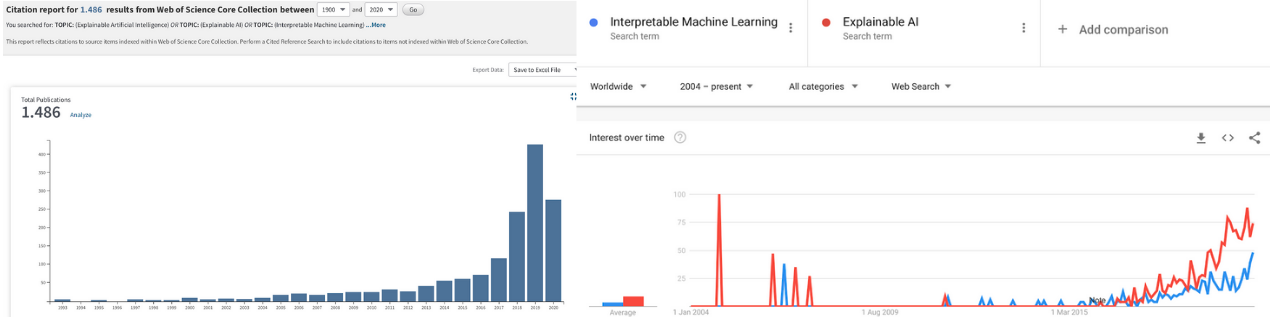
\includegraphics[width=\textwidth]{citation-search.png}
  \caption{Left, Right}
  \label{fig:count}
\end{figure}
Since then, many approaches have been introduced to the field, many of them model-agnostic explanation methods, which work for different types of ML models, but also model-specific explanation methods to interpret,for example, deep neural networks and tree ensembles.
Regression analysis and rule-based ML remain important and active research areas to this day and are blending together (e.g., model-based trees \cite{zeileis2008model}, RuleFit \cite{friedman2008predictive}).
Many extensions of the linear regression model exist \cite{hastie1990generalized,fahrmeir2013multivariate,gelman2006data} and linear regression models remain an active field of research \cite{fasiolo2020scalable,caruana2015intelligible,fasiolo2020fast,ustun2016supersparse} 
Rule-based ML also remains an active area of research (for example, \cite{wang2015falling,letham2015interpretable,hothorn2015ctree}).
Both regression models and rule-based ML serve as stand-alone ML algorithms, but also as building blocks for many other IML approaches.

\section{Today}

IML has reached a first state of usability.
Research-wise, the field is maturing in terms of methods surveys  \cite{molnar2019,guidotti2018survey,vilone2020explainable,rosenfeld2019explainability,adadi2018peeking,anjomshoae2019explainable,du2019techniques,carvalho2019machine}, further consolidation of terms and knowledge \cite{hall2019systematic,doshi2017towards,murdoch2019definitions,samek2019towards,preece2018stakeholders,chromik2020taxonomy} and work about defining interpretability or evaluation of IML methods \cite{mohseni2018multidisciplinary,mohseni2018human,ribeiro2016should,hoffman2018metrics}.
We have a better understanding of weaknesses of IML methods \cite{laugel2019dangers,molnar2019,molnar2020pitfalls,hooker2019please,adebayo2018sanity,janzing2019feature,sundararajan2019many,strobl2007bias,strobl2008conditional,apley2016visualizing}.
Open source software  with implementations of various IML methods is available \cite{iml,biecek2018dalex,pedregosa2011scikit,klaise2020alibi,nori2019interpretml} and gives ML practitioners the means to interpret their models.
Regulation such as GDPR has spurred a discussion around further needs of interpretability \cite{wachter2017counterfactual}.
IML has also arrived in industry \cite{gade2019explainable}, there are startups that focus on machine learning interpretability and also big tech companies offer software \cite{exler2019if,arya2020ai,hall2017machine}.

\section{IML Methods}

We distinguish IML methods between component and sensitivity analysis\footnote{Not to be confused with the research field of sensitivity analysis, which studies the uncertainty of outputs in mathematical models and systems. There are methodological overlaps (e.g., Shapley values), but also differences in methods and how input data distributions are handled.}, illustrated in Figure~\ref{fig:iml-type}.
An IML method that works by component analysis assigns meaning to \textit{(learned) model parameters and structures} while sensitivity analysis \textit{probes the model with artificial data points and describes its behavior}.\footnote{Some surveys distinguish between \textit{ante-hoc (alternatively: transparent design, white box models, inherently interpretable model)} and \textit{post-hoc} IML method, depending on whether interpretability is considered at model design and training or after training, leaving the (black-box) model unchanged. Another category divides model-agnostic and model-specific. Component vs. sensitivity analysis is, in our opinion, another interesting view.}

\begin{figure}
    \centering
    \begin{minipage}{0.45\textwidth}
        \centering
        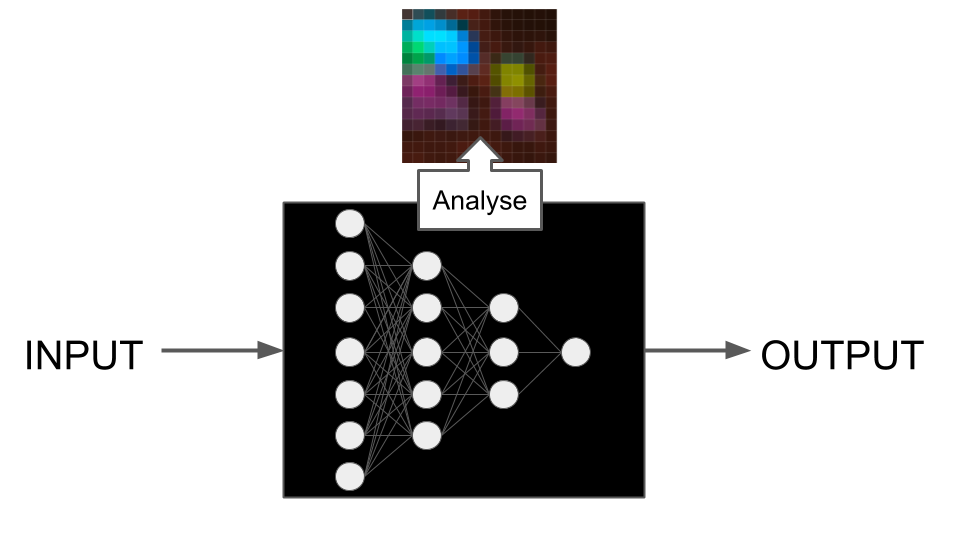
\includegraphics[width=0.9\textwidth]{specific-black-box.png}
    \end{minipage}\hfill
    \begin{minipage}{0.45\textwidth}
        \centering
        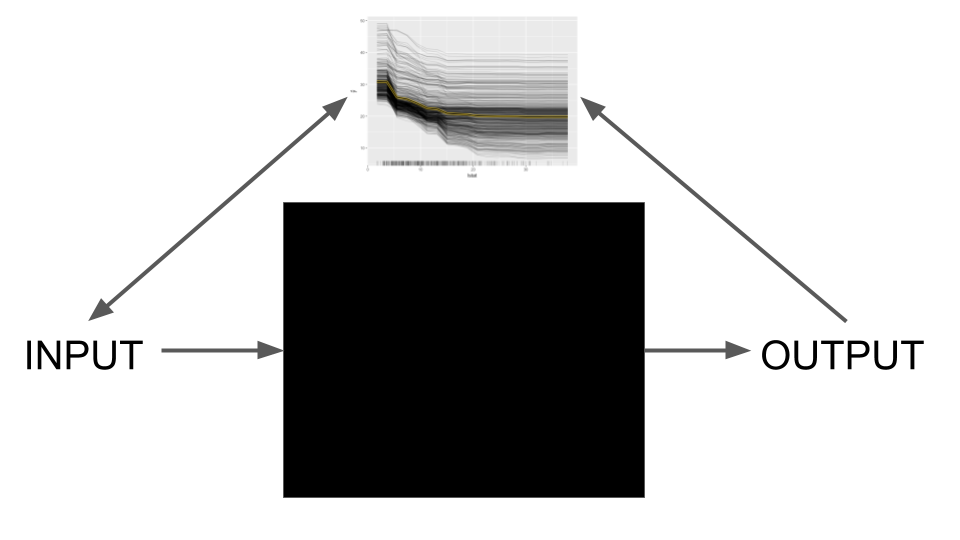
\includegraphics[width=0.9\textwidth]{agnostic-black-box.png}
    \end{minipage}
    \label{fig:iml-type}
    \caption{Some IML approaches work by assigning meaning to individual model components (left), some by analyzing the model predictions for perturbations of the data.}
\end{figure}



\subsubsection{Analyzing Components of \enquote{Interpretable} Models}
Component analysis requires that a model can be decomposed into individual components that we can interpret individually, like weights in a linear model, but it does not necessarily require that the user understands the model in its entirety (simulatability).
Component analysis is always model-specific, e.g., a linear regression model can be interpreted by analyzing its coefficients, while a decision tree can be interpreted by visualizing the learned decision structure.
\textbf{Inherently interpretable models} are models with learned structures and learned parameters which can be assigned some meaning.
Linear regression models, decision trees and decision rules are considered to be interpretable \cite{freitas2014comprehensible,huysmans2011empirical}.
%As a rule of thumb for when we do an introspection is that we are not probing the model with various (manipulated data points).
Linear regression models ($Y = \beta_0 + \beta_1 x_1 + \ldots + \beta_p x_p$) can be interpreted by analyzing components:
The model structure, a weighted sum of features, allows that we interpret the $\beta$-weights as the effect that a feature has on the prediction.
Decision trees and other rule-based ML models have a learned structure (e.g.,\enquote{IF feature $x_1 > 0$ and feature $x_2 \in \{A,B\}$, THEN predict 0.6}).
We can interpret the learned structure to trace how the model makes predictions.
The more complex interpretable models get (e.g., linear models with hundreds of features and complex interaction terms or deep decision trees), the more difficult the interpretation becomes.

\subsubsection{Analyzing Components of \enquote{Black-Box} Models}

With a bit more effort, we can also analyze components of black box models.
\footnote{This blurs the line between \enquote{inherently interpretable} and a \enquote{black-box} model.}
For example, the abstract features learned by a deep convolutional neural network (CNN) can be visualized by finding or generating images that activate a feature map of the CNN \cite{olah2017feature}.
For the random forest, the minimal depth distribution \cite{randomForestExplainer,ishwaran2010high} and the Gini importance \cite{breiman2001random} analyze the structure of the trees of the forest and can be used to quantify feature importance.
% TODO: Finde more examples to make black-box model structures interpretable. Also, e.g., the logistic regression model needs \enquote{post-hoc} analysis bc. we have to compute log odds from the weights. and for gam we have to visualize the function learned by splines
If a ML algorithm is well understood and frequently used in a community, like random forests in ecology research \cite{cutler2007random}, model component analysis can be powerful, but it has the disadvantage that it is tied to that specific model.

\subsection{Local Sensitivity Analysis}

Sensitivity analysis is mostly model-agnostic and works by manipulating input data and analyzing the respective model predictions.
IML methods based on sensitivity analysis often treat the ML model as a closed system that receives features as an input and produces the prediction as output.
In the following, we distinguish between local and global explanations.
Local methods explain individual predictions of ML models.
Local explanation methods have received much attention and there has been a lot of innovation in the last years.
Popular local IML methods are LIME \cite{ribeiro2016should}, Shapley Values \cite{lundberg2017unified,vstrumbelj2014explaining} and Counterfactual Explanations \cite{wachter2017counterfactual,dandl2020multi}.
Counterfactual explanations explain predictions in the form of what-if scenarios, which builds on a rich tradition in philosophy.
According to findings in the social sciences \cite{miller2019explanation}, counterfactual explanations are \enquote{good} explanations because they are contrastive and focus on a few reasons.
A different approach originates from collaborative game theory:
The Shapley values \cite{shapley1953value} provide an answer on how to fairly share a payout among the players of a collaborative game.
The collaborative game idea can be applied to ML \cite{vstrumbelj2014explaining,lundberg2017unified,lundberg2018consistent}:
The predicted value is the payout, each feature value is a player.
% TODO: Write about extensions and evaluations, also cite kumar2020problems. Check MOC paper for references
Another popular method are local interpretable model-agnostic explanations, short LIME \cite{ribeiro2016should}.
LIME uses surrogate models, i.e., the method trains an interpretable model such as a linear regression model to approximate the predictions of original ML model.
Numerous extensions of LIME exist, that try to fix issues with the original method, extend it to other tasks and data or analyze its properties \cite{hu2018locally,rabold2018explaining,rabold2019enriching,visani2020optilime,haunschmid2020audiolime,rahnama2019study,shankaranarayana2019alime,botari2020melime}.
% TODO: Add the many extensions of Shapley Values
% TODO: Add extensions and implementations of Counterfactual explanations
Some IML methods rely on model-specific knowledge to analyze how changes in the input features changes the output.
Saliency maps for CNNs make use of the network gradients to explain individual classifications.
The explanations are in the form of heatmaps that show how changing a pixel can change the classificaiton.
The saliency map methods differ in how they backpropagate \cite{sundararajan2017axiomatic,lundberg2017unified,montavon2017explaining,simonyan2013deep,shrikumar2016not}.
Additionally model-agnostic versions \cite{ribeiro2016should,lundberg2017unified,zeiler2014visualizing} exist for analyzing image classifiers.

\subsection{Global Sensitivity Analysis}

Global model-agnostic explanation methods are used to explain how the model behaves on average for some given dataset.
A useful distinction of global explanations are feature importance and feature effect.
Feature importance ranks features based on how relevant they were for the prediction.
Permutation feature importance \cite{fisher2019all,casalicchio2018visualizing} is a popular importance measure, originally suggested for random forests \cite{breiman2001random}.
An alternative are variance based measures.
See \cite{wei2015variable} for an overview of all the ways to measure importance.
The feature effect expresses how a change in a feature changes the predicted outcome.
Popular feature effect plots are partial dependence plots \cite{friedman2001greedy}, individual conditional expectation curves \cite{goldstein2015peeking}, accumulated local effect plots \cite{apley2016visualizing} and the functional ANOVA \cite{hooker2007generalized}.
Analyzing influential data instances, inspired by statistics, provides a different view into the model and describes how influential a data point was for a prediction \cite{koh2017understanding}.


\subsection{Surrogate Models}

Surrogate models\footnote{Surrogate models are related to knowledge distillation and the teacher-student model.} are interpretable models designed to \enquote{copy} the behavior of the ML model.
They do not neatly fit into the categorization of component or sensitivity analysis, as they combine both:
The surrogate approach treats the ML model as a black box, only requiring the input / output data  (similar to sensitivity analysis), but the interpretation is based on analyzing components of the interpretable surrogate model.
Many IML methods are surrogate model approaches \cite{puri2017magix,molnar2019,ming2018rulematrix,ribeiro2016should,frosst2017distilling,bastani2017interpreting,craven1996extracting,krishnan2017palm} and differ in the targeted ML model, the data sampling strategy, the interpretable model that is used and so on.
There are also methods for extracting, e.g., decision rules from specific models based on their internal components such as weights \cite{andrews1995survey,augasta2012rule}.

%What I missed out on:
%
%- Human-Computer Interaction, e.g. (Explainable Artificial Intelligence: a Systematic Review) sees Explainable AI as the intersection between Artificial Intelligence and Human-Computer Interaction.
%- Ethics and Philosophy.
%- Some methods are designed or adapted so that we can more easily understand what its components do. For example for neural networks we can \textit{disentangle} the individual neurons TODO:CITE, so that we can interpret them better.
%- TODO: Add more to the idea of making components of a (black-box) ML model more interpretable. This can be e.g. tree pruning, adding sparsity to linear regression models, disentangle neurons.
%- We did not touch topics where data is analyzed before modelling to understand the data better
% - Talk about social science: miller2017explainable
%This can helps component analysis, e.g., a linear model with most coefficients at zero is easier to interpret.
%But this can also help with sensitivity analysis, as PDPs of monotonic features will only show in one direction.
% TODO: Write about dependent features and how they are affecting interpretation. also cite kumar2020problems here
\section{Challenges}

This section presents an incomplete of challenges for IML, mostly based on \cite{molnar2020pitfalls}.

\subsection{Statistical Uncertainty and Inference}

Many IML methods such as permutation feature importance or Shapley values provide explanations without quantifying the uncertainty of that explanation.
The model itself, but also the explanations are computed from data and are subject to uncertainty.
We have to become more rigorous in reporting explanations including their uncertainty.
First research is working towards quantifying uncertainty of explanations, for example, for feature importance \cite{watson2019testing,fisher2019all}, layer-wise relevance propagation \cite{fabi2020feature} and Shapley values \cite{williamson2020efficient}.

With IML, with have methods to compute meaningful properties of an ML model. 
But to infer properties about the data generating process from the ML model, we have to specify the required assumptions that would allow us to do so.
We also need tools and procedures to check these assumptions.
Hopefully we can avoid problems in statistical testing, such as p-hacking \cite{head2015extent} and the resulting publication bias \cite{begg1994publication}.

\subsection{Causal Interpretation}
Ideally, a model relies on the true causes to make a prediction.
Then we could  interpret it causally, making statements about the underlying phenomena, which is the focus of ML in research, but also makes models robust against adversarial attacks, and more useful when used as a basis for decision making.
% TODO: Find citation for this statement
Unfortunately, predictive performance and causality can be conflicting goals.
For example, today's weather directly causes tomorrow's weather, but we might only have access to feature \enquote{wet ground}.
Using \enquote{wet ground} in the prediction model for \enquote{tomorrow's weather} is useful as it has information about \enquote{today's weather}, but we are not allowed to interpret it causally, because the confounder \enquote{today's weather} is missing from the ML model.
Further research is needed to understand when we are allowed to make causal interpretations of an ML model.
First steps have been made for permutation feature importance \cite{konig2020relative} and Shapley values \cite{ma2020predictive}.

\subsection{Feature Dependence}

Feature dependence introduces problems with attribution and extrapolation.
% Attribution problem
Attribution of importance and effects to features becomes difficult when features are, for example, correlated and therefore share information.
It can be shown that correlated features in random forests are preferred and attributed a higher importance \cite{strobl2008conditional,hooker2019please}.
% Extrapolation problem
Many sensitivity analysis based methods permute features.
When the permuted feature has some dependence with another, this association is broken and the resulting data point extrapolates to areas outside the distribution.
The ML model was never trained on such combinations and will likely not be confronted with similar data points for realistic prediction.
Therefore extrapolation can cause misleading interpretations.
% Fixes
There have been attempts to \enquote{fix} permutation-based method, by using a conditional permutation scheme that respects the joint distribution of the data.
The change from unconditional to conditional permutation changes the respective interpretation methods \cite{molnar2020model,apley2016visualizing} or in worst case can break it \cite{janzing2019feature,sundararajan2019many}.


\subsection{Definition of Interpretability}
A lack of definition is a common critique of the field \cite{lipton2018mythos,doshi2017towards}.
Without a definition of "interpretability", how can we decide if a new method explains ML models better?
To evaluate the \textbf{predictive performance} of an ML model, we simply compute the prediction error on test data given the groundtruth label.
To evaluate the \textbf{interpretability} of that same ML model is more difficult.
We do not know what the groundtruth explanation looks like and have no straightforward mean to quantify how interpretable a model is or how correct an explanation is.
Instead of having one groundtruth explanation, various \textbf{quantifiable aspects of interpretability} are emerging \cite{poursabzi2018manipulating,philipp2018measuring,molnar2019quantifying,hauenstein2018computing,zhou2018measuring,akaike1998information,schwarz1978estimating,poursabzi2018manipulating,dhurandhar2017tip,friedler2019assessing}.

The two main ways of evaluation of interpretability are: \textbf{objective evaluations} which are mathematically quantifiable metrics, and {human-centered evaluations} which involve studies with users.
Examples of aspects of interpretability are sparsity, interaction strength, fidelity (how well explanation approximates the ML model), sensitivity to perturbations, and a user's ability to run a model on a given input (simulatability).
% TODO: check with IML book
The challenge ahead remains to establish a best practice on how to evaluate interpretation methods and the explanations they produce.
Here we should also look to the field of Human-Computer Interaction who do exactly that.

\subsection{More Challenges Ahead}
% TODO: Rework section
We have focused mostly on the methodological, mathematical challenges in a rather static setting, where you are given a machine learning model and data.
But ML models are not used in a static and isolated way.
Rather they are embedded in a process or product.
What is the best way to explain a machine learning model for people with a specific background and how do we present the explanations?
How are people affected by explanations, how are explanations maybe misused?
This is also a rather static view point in the sense that we can do a lot if we allow a more interactive way of modeling and "having a conversation" between a person and the model or even the modeling process.
How do we present multiple maybe conflicting explanations, e.g., when you generate multiple counterfactual explanations?

\section{Discussion}

Interpretable machine learning is a young field, but has deeper roots in statistics and computer science and also draws from other fields such as the social sciences, human-computer interaction and game theory.
There has been a Cambrian explosion of methods in the 2010s, including model-agnostic interpretation methods and many specialized methods for, e.g., deep neural networks.
Many IML methods have found their way into open source software and products of startups and tech companies.
Interpretable machine learning is used in science, company products and processes.
While we have reached a first state of usability and productivity, there a still some challenges ahead, such as feature dependence, causality and uncertainty quantification.
To solve the challenges ahead, we believe that the field has to reach out horizontally -- to other domains -- and vertically -- drawing from the rich research in statistics and computer science.


%
% ---- Bibliography ----
%
% BibTeX users should specify bibliography style 'splncs04'.
% References will then be sorted and formatted in the correct style.
%
% \bibliography{mybibliography}
%

\vskip 0.2in
\bibliographystyle{splncs04}
\bibliography{Bib}

\end{document}
